\section{Experiments}
%
In this section we describe the experiments carried out in order to assess 
the performance and the behavior of our extended kitchen sinks (\eks) and 
unscented kitchen sinks (\uks) methods. We first look at experiments on 
small-scale synthetic inversion problems and a binary classification task on 
the \usps dataset. As these experiments were also carried out by 
\citet{steinberg-bonilla-nips-2014} to evaluate the \egp and the \ugp, 
our first goal  is to investigate how well 
random kitchen sinks basis can approximate the original \egp and \ugp.
Additionally, we are interested in determining whether the complexity 
of the algorithms  can be reduced significantly by having a smaller number 
of basis functions than the number of training points.
%
\subsection{Synthetic Inversion Problem}
In this experiment we generate latent function values ($\latents$) from a
Gaussian process with isotropic squared exponential covariance function (having
a signal variance  $\sigma^2_s = 0.8^2$ and a length-scale $\ell = 0.6$) at
1000 input points, $\ins \in \real{}$, which are uniformly spaced between
$[-2\pi, 2\pi]$. We test our algorithms and the baselines (\ugp, \egp) with
five simple forward models; an identity function (linear), a 3rd order
polynomial with no cross terms (poly3), an exponential function, a sinusoid,
and a tangent function. We present the results of 5-fold cross validation (200
training, 800 testing) in Table \ref{tab:toyinversions}, and we also experiment
with the number of basis functions for the \eks and \uks in
Figure \ref{fig:toyinversions}. As in \citet{steinberg-bonilla-nips-2014} we
use standardized mean square error (SMSE) and negative log probability density
(NLPD) as the performance metrics.
%
\begin{table}[h]
\caption{Performance of the \eks and \uks methods compared to their GP counterparts (\egp and \ugp) on a range of synthetic benchmarks. 
\gp the corresponds to the GP analytical solution in the linear case.
\todo{PUT GP baseline}
\label{tab:toyinversions}
}

\begin{center}
\begin{scriptsize}
\begin{tabular}{c c c c c}
g(f) & Method & SMSE-f* (std) & NLPD-f* (std) &SMSE-g* (std) \\ 
\toprule
linear & \eks & 0.0338 (0.0180) & -1.0382 (0.2664) & 0.0338 (0.0180) \\ 
& \uks & 0.0338 (0.0180) & -1.0383 (0.2663) & 0.0338 (0.0180) \\ 

& \egp & 0.0324 (0.0146) & -1.0105 (0.2995) & 0.0324 (0.0146) \\ 
& \ugp & 0.0345 (0.0176) & -0.9392 (0.4295) & 0.0345 (0.0176) \\ 

poly3 & \eks & 0.0157 (0.0031) & -1.4258 (0.1514) & 0.0045 (0.0008) \\ 
& \uks & 0.0140 (0.0027) & -1.4488 (0.1663) & 0.0045 (0.0009) \\ 

& \egp & 0.0671 (0.0247) & -0.3596 (0.6799) & 0.0164 (0.0053) \\ 
& \ugp & 0.0579 (0.0360) & -0.3544 (0.6156) & 0.0138 (0.0085) \\ 

exp & \eks & 0.0293 (0.0123) & -1.2410 (0.1819) & 0.0132 (0.0045) \\ 
& \uks & 0.0218 (0.0072) & -1.2693 (0.2069) & 0.0116 (0.0022) \\ 

& \egp & 0.0820 (0.0419) & 0.2480 (1.5229) & 0.0367 (0.0223) \\ 
& \ugp & 0.0342 (0.0220) & -1.0185 (0.5768) & 0.0167 (0.0112) \\ 

sin & \eks & 0.0391 (0.0141) & -0.9706 (0.1508) & 0.0342 (0.0090) \\ 
& \uks & 0.0252 (0.0049) & -1.1592 (0.0864) & 0.0261 (0.0055) \\ 

& \egp & 0.0405 (0.0202) & -0.9373 (0.2509) & 0.0374 (0.0228) \\ 
& \ugp & 0.0554 (0.0236) & -0.8044 (0.2175) & 0.0509 (0.0259) \\ 

tanh & \eks & 0.0598 (0.0225) & -1.0856 (0.1461) & 0.0230 (0.0047) \\ 
& \uks & 0.0449 (0.0281) & -1.2922 (0.2163) & 0.0272 (0.0252) \\ 

& \egp & 0.0881 (0.0560) & -0.8520 (0.2398) & 0.0394 (0.0242) \\ 
& \ugp & 0.0504 (0.0290) & -0.8676 (0.2242) & 0.0344 (0.0127) \\ 

\bottomrule
\end{tabular}

\end{scriptsize}
\end{center}
\end{table}
%
\begin{figure*}
\centering
\begin{tabular}{c c c}
\includegraphics[width=0.31\linewidth]{toyData-EKS-SMSE-fstar} &
\includegraphics[width=0.31\linewidth]{toyData-EKS-NLPD-fstar} &
\includegraphics[width=0.31\linewidth]{toyData-EKS-SMSE-gstar} \\
\includegraphics[width=0.31\linewidth]{toyData-UKS-SMSE-fstar} &
\includegraphics[width=0.31\linewidth]{toyData-UKS-NLPD-fstar} &
\includegraphics[width=0.31\linewidth]{toyData-UKS-SMSE-gstar} \\
\end{tabular}
\caption{The performance of the \eks (top) and \uks (bottom)
on the synthetic inversion problems as a function of the number of features used. 
\label{fig:toyinversions}
}
\end{figure*}
%
%%%%%%%
\subsection{Binary Handwritten Digit Classification}
Figure \ref{fig:usps}

\begin{figure*}[h]
\centering
\begin{tabular}{c c}
\includegraphics[width=0.45\linewidth]{uspsData-NLP}  &
\includegraphics[width=0.45\linewidth]{uspsData-ERROR-RATE}  
\end{tabular}
\caption{The performance of the \eks and \uks (bottom) on the binary classification problem for the \usps dataset as a function of 
the number of  basis used. \egp and \ugp are the original (full) \gp models.
\label{fig:usps}
}
\end{figure*}
%
%%%%%%%%%
\subsection{Large Scale Classification}
Table \ref{fig:mnistBinary}
Here we show the results on \mnist dataset.
\begin{table}[h]
\caption{The performance of the models on the \mnist dataset for the 
task of classifying the even digits vs the odd digits.
\label{fig:mnistBinary}
}
\begin{tabular}{c c c c c}
\toprule
& \multicolumn{2}{c}{NLP} & \multicolumn{2}{c}{Error Rate} \\
& D = 1000 & D = 2000 & D = 1000 & D = 2000 \\
\midrule
\eks &  0.129 & 0.088 & 0.043 & 0.026 \\
\uks &  0.129 & 0.088 & 0.043 & 0.026 \\
\hmg &      \multicolumn{2}{c}{0.069}    &            \multicolumn{2}{c}{0.022}   \\
\dnb   &      \multicolumn{2}{c}{0.068}    &            \multicolumn{2}{c}{0.022}\\
\bottomrule
\end{tabular}
\end{table}

\hmg refers to \citet{hensman-et-al-aistats-2015} 
\dnb refers to \citet{dezfouli-bonilla-nips-2015}

\subsection{Seismic Inversion}

In this experiment we demonstrate the \eks and \uks performing a
one-dimensional seismic inversion. The goal is to infer both the geometry of
the interfaces between subsurface geological layers and the seismic propagation velocity
within each layer from noisy, interpreted surface observations of sound
reflection times, \Outs. We use two datasets for this experiment; a simulated
world with two randomly generated splines representing geological layers (providing a ground-truth), 
and a real seismic line from the Otway basin in South Australia (Pretty Hill
formation) providing reflection times for the four main layer formations.
Each dataset has 50 and 113 observations per layer respectively.

The inputs, $\Ins$, are the surface locations (metres) of the seismic sensors,
and we use the following forward model,
\begin{align}
    \latents_p^\text{depth} &= \max\cbrac{\latents_p^\text{depth, input},
        \latents_{p-1}^\text{depth}} \quad \forall p, \label{eq:clip} \\
    \nonlinf_p^\text{time} &=
    \begin{cases}
        2\frac{\latents_p^\text{depth} - \latents_{p-1}^\text{depth}}
        {\latents_p^\text{vel}} + \nonlinf_{p-1}^\text{time},
        & \text{if } p > 0 \\
        2\frac{\latents_0^\text{depth}}{\latents_0^\text{vel}},
        & \text{if } p = 0
    \end{cases}
\end{align}
Where there are $\otdim$ output tasks -- reflection times from each layer,
$\nonlinf_p^\text{time}$, and there are two types of latent input tasks;
\begin{itemize}
    \item $\latents_p^\text{depth}\!\brac{\Ins}$, the geological depth of layer
        $p$ corresponding to each surface location. Equation \eqref{eq:clip} 
        clips overlapping estimated (input) layers to create these valid
        layers.
    \item $\latents_p^\text{vel}\!\brac{\Ins}$, the velocity of layer $p$ 
        corresponding to each surface location.
\end{itemize}

Each of these input tasks corresponds to an output task, so we have also
indexed by $p$ instead of $q$. Naturally then $\ltdim = 2\otdim$, and the
problem is under-constrained since there is an infinite set of layer depths and
velocities that can generate the reflection times. To help constrain our
models, we put a prior on the average depth of each layer.

We compare against two baseline methods. The first baseline applies
gradient-free optimisation to identify the maximum a-posteriori latent tasks.
A GMRF prior is used to model the deviation of each layer from a flat mean
function.

The second baseline is a probabilistic approach using MCMC to sample from
the posterior distribution. For this implementation, the dimensionality of the 
inference problem has been reduced by parameterising the latent tasks as 
truncated cosine basis functions located on a regular grid, such that the MCMC
learns the distribution of their weights. We have used 20 parameters per
latent task, plus one observation noise variance parameter for each of the four 
observed taks. Independent Gaussian priors are placed on the basis weights, and 
a Gamma prior on each of the per-task observation variances.

\begin{figure}
\includegraphics[width=0.4\textwidth]{seismicData-depth-Taylor-1000} \\
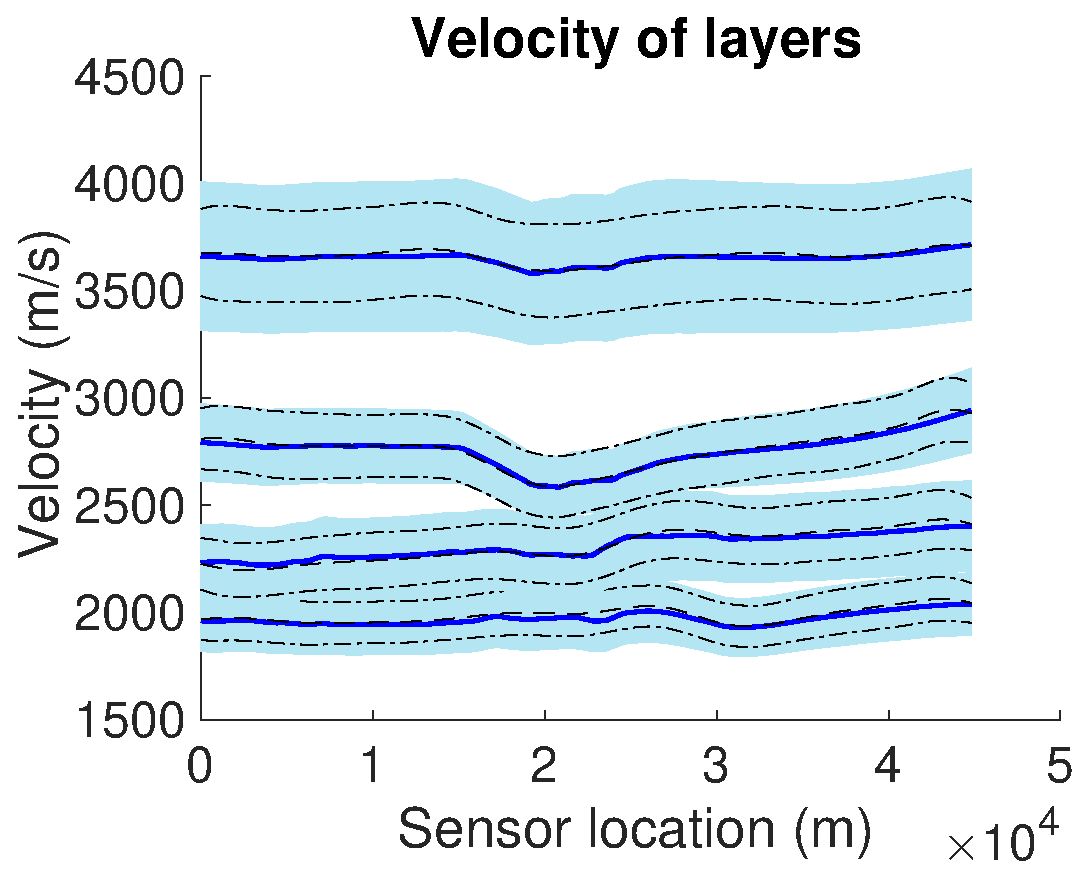
\includegraphics[width=0.4\textwidth]{seismicData-vel-Taylor-1000}
\caption{The inferred layer boundaries (top) seismic velocities on
 on the seismic inversion problem. }
\end{figure}

\fix{TODO}:
\begin{itemize}
    \item NLPD and MSE on the simulation data
    \item Plot of the Otway data
\end{itemize}


